\chapter{Implementazione\label{sec:implementazione}}
In questa sezione verranno descritte tutte le tecnologie utilizzate per lo sviluppo dell'applicazione.
\section{Ambiente di sviluppo\label{sec:ambiente}}
%TODO aggiungere info relative a pc e strumenti usati, sistemi operativi, dispositivi, eccetera
Per lo sviluppo dell'applicazione è stato utilizzato il sistema di controllo di versione Git,  la realizzazione del progetto è stata eseguita da i seguenti calcolatori:
\begin{itemize}
	%\item OS: Windows 10 Home 64 bit , CPU: Intel Core i7-3630QM, RAM 8.00 GB
	%oppure con meno dettagli
	%TODO controllare
	\item OS: Windows 10 Home 64bit , Ubuntu 16.04, MacOS Catalina
	\item IDE: Microsoft Visual Studio Code, Android Studio, XCode
\end{itemize}
\section{Il framework Flutter\label{sec:flutter}}
\subsection{Decrizione\label{sec:flutter-descrizione}}
Flutter è un framework cross-platform cross-compiled realizzato da Google, permette di realizzare applicazioni native eseguibili sia su Android che su iOS realizzando un singolo progetto in linguaggio Dart. La principale caratteristica di Flutter è che la User Interface è composta unicamente da componenti Widget immutabili. I widget possono definire elementi strutturali (barre, pulsanti, menù), stilistici (font, colori) o di layout (padding), e così via; in pratica ''tutto è un Widget''. Possono essere StatefulWidget, ovvero possedere uno stato ed essere quindi in grado di rispondere alle interazioni dell'utente, oppure StatelessWidget ovvero elementi statici. 
\\Flutter è realizzato in C, C++, Dart e dal motore grafico Skia. Le componenti vengono definite in Dart e renederizzate grazie ad un motore implementato in C++ che utilizza le librerie grafiche Skia. Il codice Dart viene compilato in codice nativo utilizzando la compilazione AOT (ahead-of-time) e viene eseguito grazie alla Dart Virtual machine, il motore C/C++ invece viene compilato con NDK Android o con LLVM (Low Level Virtual Machine) in iOS, permettendo la compilazione in codice nativo.
\begin{figure}[H]
	\centering
	\captionsetup{justification=centering}
	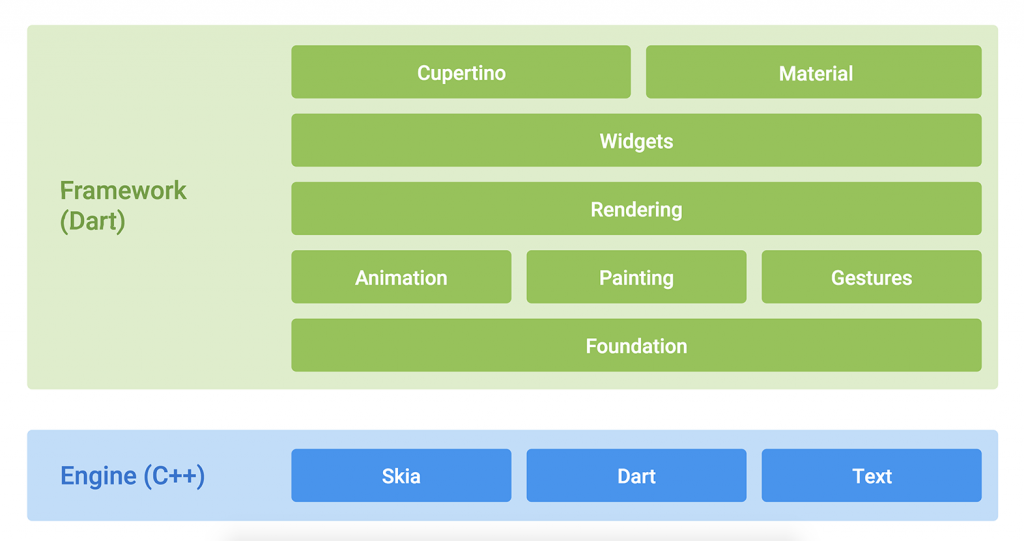
\includegraphics[width=1\linewidth]{./immagini/flutter_architecture.png}
	\caption{Architettura di Flutter}
\end{figure}

\subsection{Vantaggi e svantaggi\label{sec:flutter-vantaggi}}
I principali vantaggi che il framework Flutter possiede sono:
\begin{itemize}
	\item \textbf{Hot reload}: consente di vedere e testare rapidamente i cambiamenti eseguiti sul codice mentre l'applicazione è in esecuzione, quindi velocizza lo sviluppo;
	\item \textbf{Widgets}: possono essere utilizzati facilmente e sono definiti in stile Material design e Cupertino permetto quindi la realizzazione di un interfaccia espressiva e flessibile e la loro riusabilità rende lo sviluppo più rapido; 
	\item \textbf{Performance native}: il framework essendo cross-compiled garantisce performance al livello di app native;
	\item \textbf{Documentazione}: Flutter è ben documentato e possiede una community di utilizzatori attiva, inoltre è facilmente integrabile con Google Firebase il quale fornisce una rapida implementazione per l'archiviazione dei dati dell'applicazione e delle funzionalità di autenticazione degli utenti;
	\item \textbf{Facilmente integrabile in diversi ambienti di sviluppo}: sono disponibili vari plugins per il supporto in diversi IDE.
\end{itemize}
\subsection{Comparazione con altri framework\label{sec:flutter-comparazione}}
\lettrine[findent=1.5em]{T}odo.

\section{Strumenti di test usati}
%TODO parlare degli fantastici strumenti di Flutter se riusciremo a usarli

\section{Performance}
%TODO verificare quante risorse usiamo e quanta batteria mangiamo